\section{Marco Teórico}

	En este capítulo primeramente se explica que características presenta un boomerang durante su vuelo para que este sea capaz de regresar al lanzador. Se derivan las ecuaciones de movimiento del boomerang y como estás pueden ser integradas fácilmente para obtener la trayectoria de vuelo, los efectos de la gravedad actuando sobre el boomerang son considerados, además se muestra como se agregan los efectos del viento en las ecuaciones de movimiento.

	\subsection{Boomerangs desde un punto de vista físico}

	En esta sección se tratarán conceptos y fenómenos relacionados con el funcionamiento básico del boomerang, los cuales permitirán comprender de manera general la física asosiada a este.

		\subsubsection{Comportamiento de boomerangs de retorno}

	Recordando el concepto, los boomerangs son objetos que, al ser lanzados apropiadamente, vuelan girando rapidamente a través del aire y regresan cerca del punto de lanzamiento \cite{Hess1975} (en este documento no se considerarán los boomerangs de no retorno).

	Un boomerang de retorno (diestro) típico es lanzado en plano vertical (o ligeramente inclinado con su parte superior alejada del lanzador); en dirección horizontal (o ligeramente elevada); y con giro considerable. Al inicio, la trayectoria del boomerang sigue la dirección del vector de velocidad inicial aplicado, pero pronto presenta un desvío a la izquierda y hacia arriba, traza un bucle amplio, se acerca al lanzador y puede descender en algún lugar cerca de los pies de este, o describir un bucle más pequeño antes de tocar el suelo. Generalmente, el plano de rotación del boomerang se ``acuesta'' gradualmente de tal manera que puede estar horizontal al final del vuelo.

		\subsubsection{Lanzamiento}

	Los boomerangs de retorno pueden tener diversas formas, pero siempre consisten en dos o más brazos descansando aproximadamente en un plano. Una caracteristica escencial es la sección transversal de cada brazo, la cual es mas convexa en un lado que en otro.

	Un boomerang es lanzado sujetandolo de uno de sus extremos con el lado más convexo cerca  de la mejilla del lanzador y arrojandolo hacia adelante de manera que es liberado con un giro rápido respecto a su centro de masa (perpendicular al plano de lanzamiento).

			\begin{figure}[ht]
			\begin{center}
			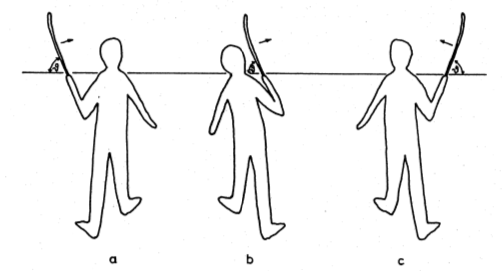
\includegraphics[scale=0.5]{imagenes/3-boomerang/Lanzamiento.png}
			\caption{Vista trasera de un lanzador (Tomada de \cite{Hess1975}).}
			\label{fig1}
			\end{center}
			\end{figure}

	En la Fig. \ref{fig1} se puede observar el ángulo $\vartheta$, es cual es el ángulo entre el boomerang y la horizontal y destacan tres tipos de lanzamientos:

		\begin{enumerate}[a)]
		\item Lanzador zurdo lanzando un boomerang zurdo,
		\item Lanzador diestro lanzando boomernag zurdo y
		\item Lanzador diestro lanzando boomerang diestro.
    	\end{enumerate}

	El ángulo $\vartheta$  entre el plano de lanzamiento del boomerang y el horizonte (vease la Fig. \ref{fig1}) tiene gran influencia en la trayectoria de vuelo. La mayoría de los boomernangs deben ser lanzados con un ángulo $\vartheta$  de entre 45 y 90 grados. Si un boomerang es lanzado a ángulos menores, generalmente describe una trayectoria ascendente y finalmente cae al suelo a gran velocidad.

		\subsection{ Los principios del boomerang de retorno}

	Aquí se presenta un modelo elemental del funcionamiento del boomerang de retorno.

	Una característica escencial del boomerang es la forma de la sección transversal de sus brazo (o aspa). Estas tienen forma de ala de avión (o de ave). Si un aeroplano vuela horizontalmente a través del aire, su peso debe ser contrarrestado por una fuerza de empuje que lo sostenga, o de otra manera caería al suelo. Esta fuerza surge de la interacción del viento con las alas del avión.

		\begin{figure}[ht]
		\begin{center}
		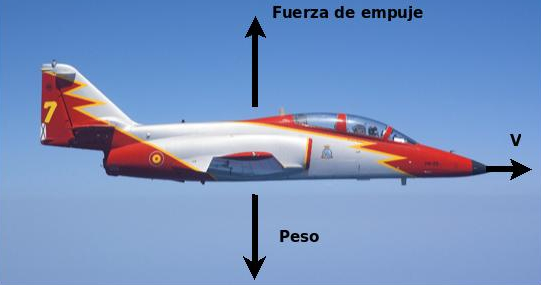
\includegraphics[scale=0.4]{imagenes/3-boomerang/plane.jpg}
		\caption{Aeroplano volando horizontalmente a velocidad V. El peso es cotrarrestado por una fuerza aerodinámica de empuje.}
		\label{fig2}
		\end{center}
		\end{figure}

	Las alas del boomerang, como las del avión tienen una forma especial que produce fuerzas aerodinámicas casi perpendiculares a la dirección de estas.

	Recuerdese que se mencionó que el brazo del boomerang presenta una cara más convexa que la otra  (lo cual es también el mismo caso de los aviones).

	La interacción del aire con la sección más convexa genera una presión del aire más baja que la producida por su contra parte. La diferencia de presiones produce una fuerza resultante de empuje, como se puede ver en la Fig. \ref{fig3}.a. Además, si el ala es inclinada más y más, la fuerza resultante se vuelve más grande Fig. \ref{fig3}.b.

		\begin{figure}[ht]
		\begin{center}
		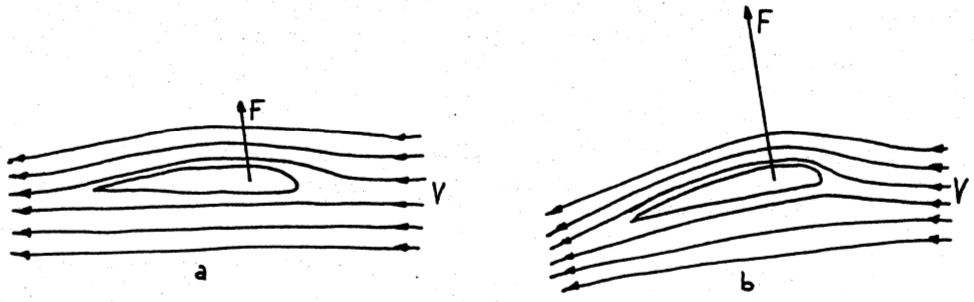
\includegraphics[scale=0.3]{imagenes/3-boomerang/airFlow.png}
		\caption{Flujo de aire alrededor de ala. F es la fuerza resultante. a: Sin inclinación aparente. b: con inclinación adicional.}
		\label{fig3}
		\end{center}
		\end{figure}
\newpage
    Recordemos que un boomerang de retorno diestro es lanzado usualmente de tal manera que su plano de rotación es casi vertical con el lado más convexo hacia la izquierda. Por tanto se produce una fuerza de empuje del lado menos convexo al más convexo, es decir, hacia la izquierda (Fig. \ref{fig4}), la cual acelera al boomerang en dicha dirección.\\\\

		\begin{figure}[ht]
		\begin{center}
		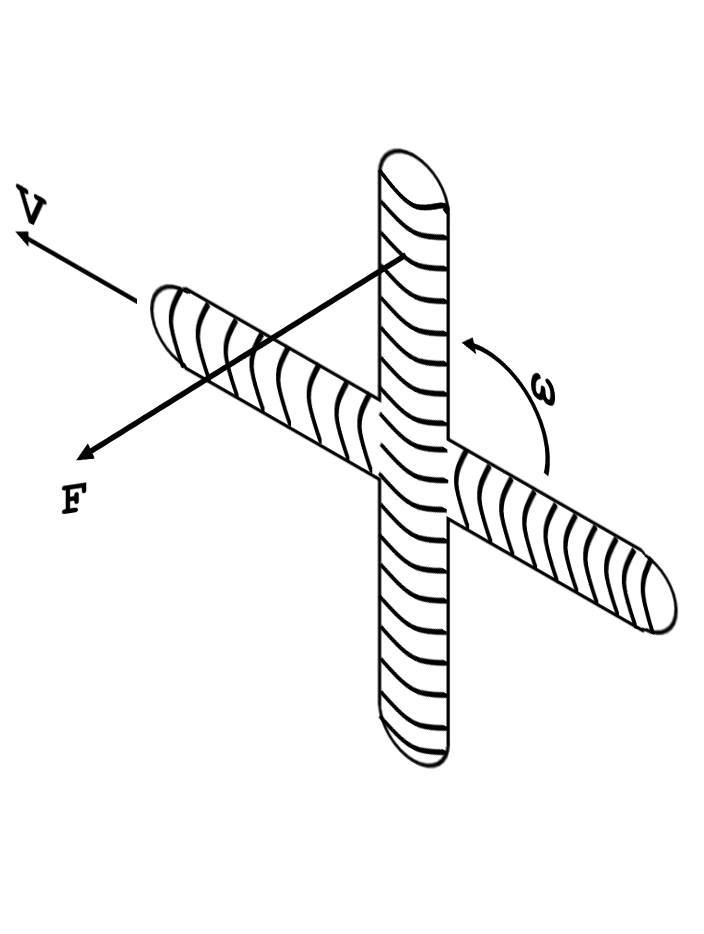
\includegraphics[scale=0.25]{imagenes/3-boomerang/leftwardForce.png}
		\caption{Fuerza resultante hacia la izquierda para boomerang diestro.}
		\label{fig4}
		\end{center}
		\end{figure}

	En adelante, particularizaremos por conveniencia a boomerangs diestros de cuatro palas (brazos). El centro de masa (CM) se encuentra en el punto de unión de sus cuatro alas y la distancia de este a cada una de las puntas es a. Se presenta una velocidad de avance $(V)$ y una velocidad angular $(\omega)$. A cada instante, no todas las particulas del boomerang tienen la misma velocidad, lo cual es resultado de la combinación de V y w.

		\begin{figure}[ht]
		\begin{center}
		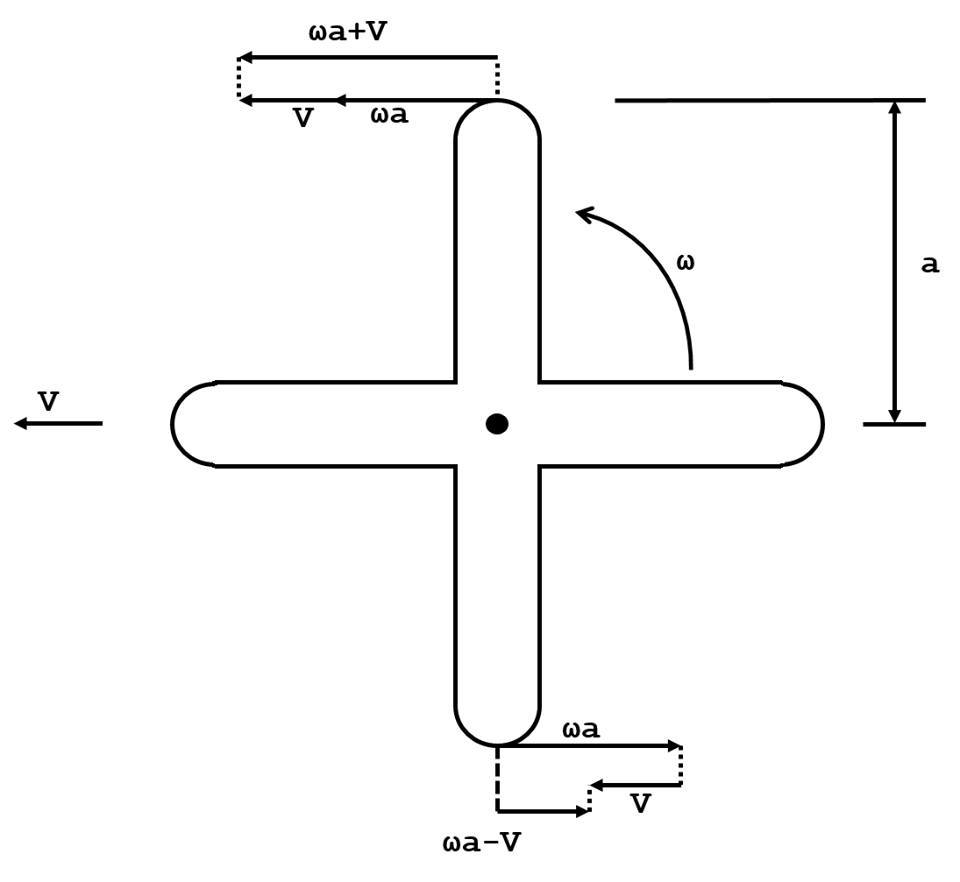
\includegraphics[scale=0.205]{imagenes/3-boomerang/upwardPointingEndofBoomerang.png}
		\caption{Velocidad de avance en los extremos superior e inferior del boomerang.}
		\label{fig5}
		\end{center}
		\end{figure}

	La punta superior del boomerang se mueve más rapido que la inferior debido a que en la primera tenemos una velocidad $V+wa$ y en la segunda tenemos $V-wa$. Generalizando tenemos que toda particula superior presenta una fuerza mayor de empuje hacia la izquierda del plano de rotación que cualquier inferior. Por lo tanto, las fuerzas aerodinamicas no solo producen una fuerza neta , sino también un par T que trata de inclinar el boomerang por su parte superior hacia la izquierda (Fig. \ref{fig6}). Esta inclinación seria respecto a un eje horizontal imaginario, llamado eje de torción, sin embargo, dicha torción no se aprecia en un boomerang.

		\begin{figure}[ht]
		\begin{center}
		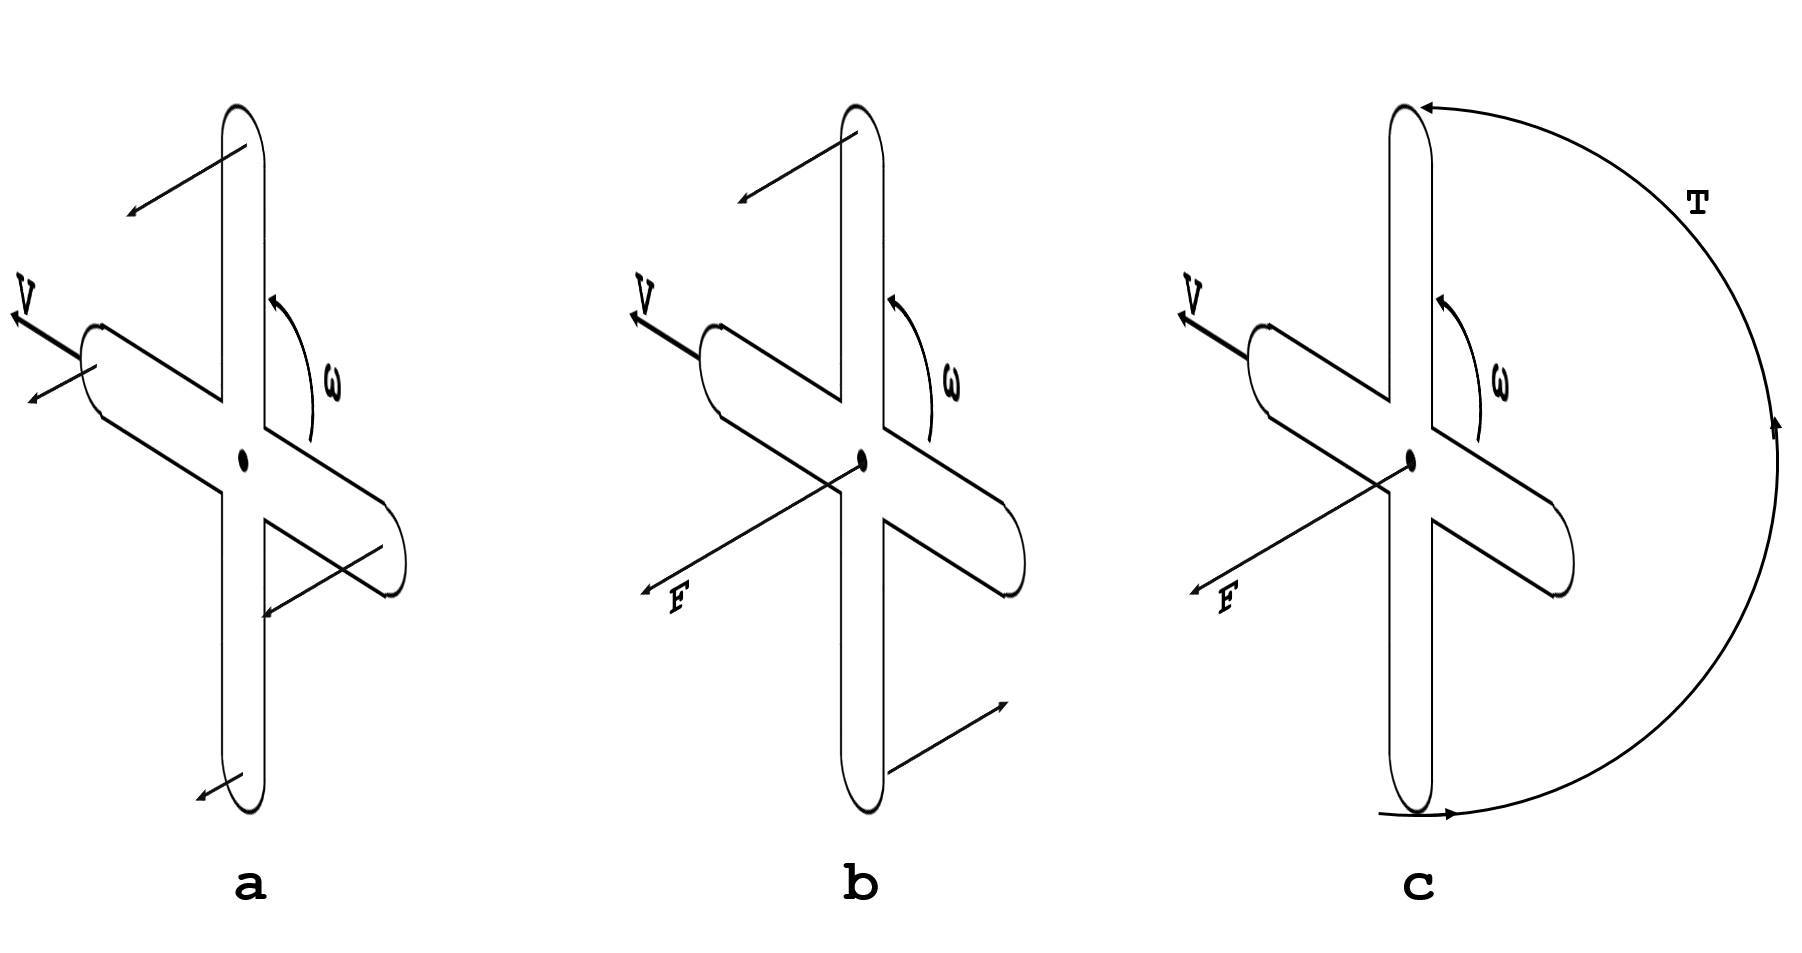
\includegraphics[scale=0.15]{imagenes/3-boomerang/DistrutionOfLEftwardForces.png}
		\caption{a: Distribución de fuerzas izquierdas. b: Fuerzas equivalentes actuando en el centro y los extremos superior e inferior del boomerang. c: Las fuerzas forman un par T, el cual trata de rotar el boomerang de su parte superior hacia la izquierda.}
		\label{fig6}
		\end{center}
		\end{figure}
\newpage
	Ahora introduciremos el concepto de movimiento de precesión:

	Pon un trompo sobre su punta y logicamente caera, pero inducele un giro rápido y se mantendra en pie. Un trompo en rotación reacciona de una manera peculiar a un par aplicado: No cede al par, en cambio rota despacio respecto a un eje imaginario perpendicular a los ejes de rotación y torción \cite{Hess1975}. Este efecto se define como ``movimiento de precesión''.

	Debido a la combinación del par generado por las fuerzas aerodinámicas y su rápida rotación, el boomerang presenta un movimiento de precesión respecto a un eje imaginario perpendicular a los ejes de rotación y de torsión.

	Si se considera un boomerang diestro al inicio del vuelo, su eje de rotación es horizontal hacia la izquierda y el eje de torsión horizontal hacia atras, por tanto, este rota (con una velocidad angular $\omega$) hacia la izquierda su parte delantera en lugar de la superior debido al efecto de precesión (Vease Fig. \ref{fig7}).

		\begin{figure}[ht]
		\begin{center}
		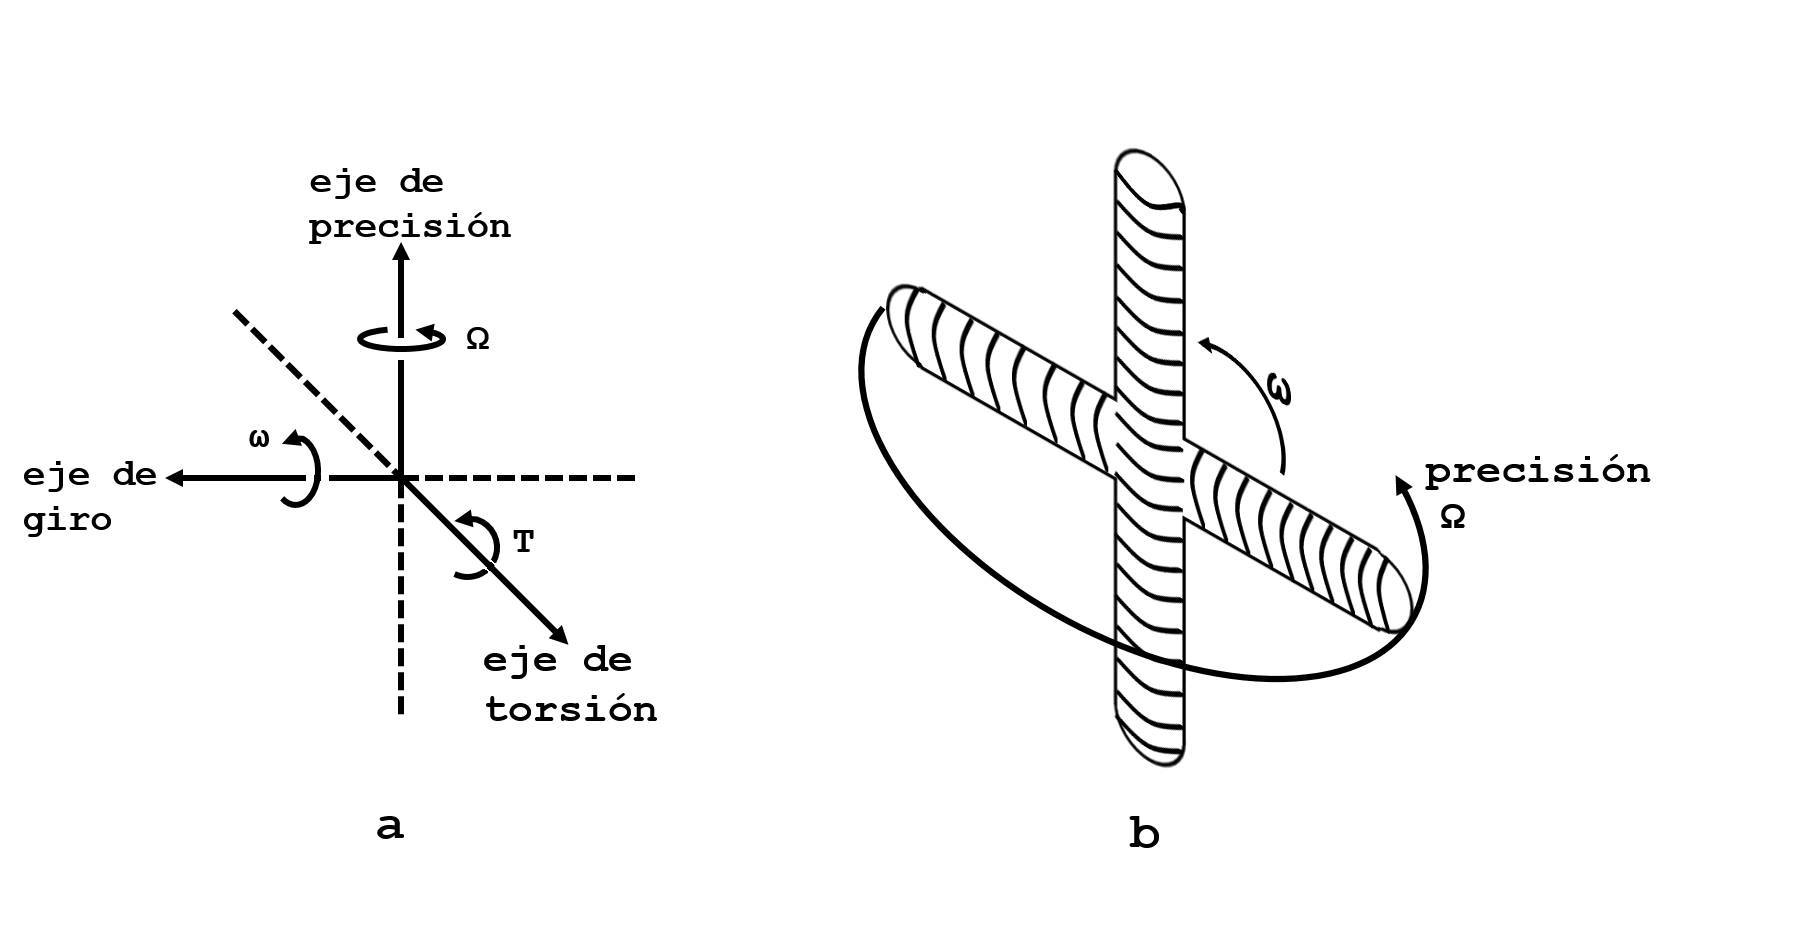
\includegraphics[scale=0.25]{imagenes/3-boomerang/precesionAlrededorDeOmega.png}
		\caption{a) Precesión $\Omega$ con respecto a un eje perpendicular a al eje de torción y el eje de rotación. b) Precesión del boomerang.}
		\label{fig7}
		\end{center}
		\end{figure}

	Para entender mejor el efecto de precesión, observese la Fig. \ref{fig8}. Podemos descartar la fuerza neta resultante en el centro de masa debido a que su único efecto es acelerar el boomerang hacia la izquierda. El par T es originado por las fuerzas de la parte superior e inferior, de igual magnitud y con sentido opuesto (vease Fig. \ref{fig5}). La maxima fuerza izquierda es ejercida por la punta superior (Fig. \ref{fig8}.a), la cual es acelerada gradualmente hasta alcanzar una velocidad, la cual alcanza su valor máximo cuando este punto se convierte en la punta frontal (Fig. \ref{fig8}.b). Cuando esta parte desciende más, el par T empieza a empujarla hacia la derecha, lo cual decrementa su velocidad. La fuerza derecha máxima se presenta cuando la punta considerada está en el punto más bajo (Fig. \ref{fig8}.c), donde la velocidad izquierda ha desaparecido y la velocidad derecha comienza a crecer, alcanzando su punto máximo a mitad del camino al punto superior (Fig. \ref{fig8}.d), y se desvanec al completar una revolución (Fig. \ref{fig8}.a). El resultado de esta secuencia es indicado en la Fig. \ref{fig8}.e.


	La combinación de velocidad hacia la izquierda en la parte frontal y velocidad hacia derecha en la parte posterior constituye el movimiento de precesión, es decir, el boomerang rota su plano respecto a un eje imaginario vertical. A mayor par, una precesión más rápida.

		\begin{figure}[ht]
		\begin{center}
		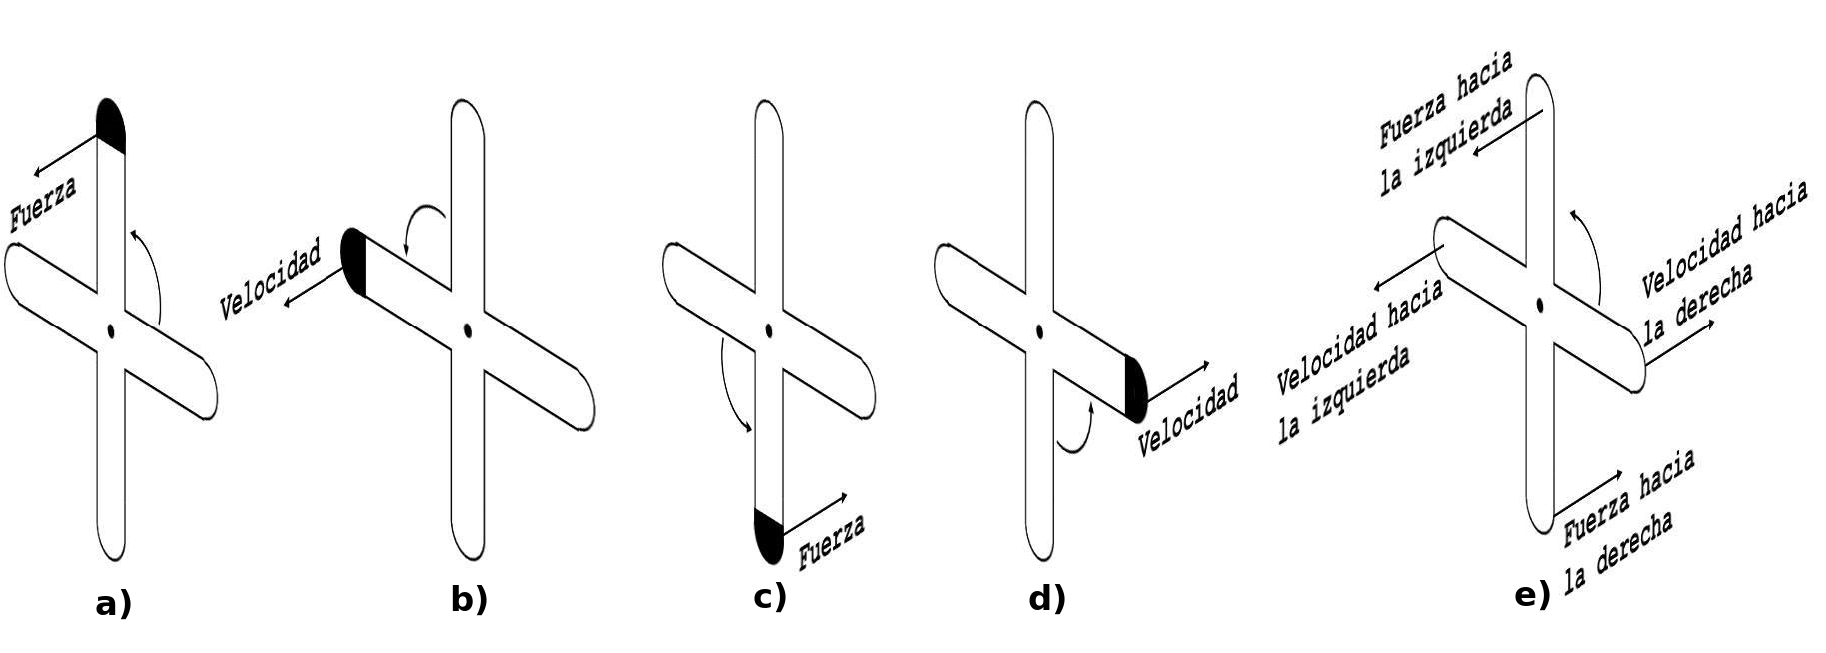
\includegraphics[scale=0.15]{imagenes/3-boomerang/PrecesionDelBoomerang.png}
		\caption{Precesión del boomerang. a,b,c,d: puntas del boomerang durante el transcurso de la revolución. e: La parte frontal tiene una velocidad hacia la izquierda, y la parte posterior hacia la derecha.}
		\label{fig8}
		\end{center}
		\end{figure}

	Ahora llamemos $\Psi$ al angulo entre el plano de rotación del boomerang y la dirección de su velocidad de avance V. Si $\Psi$ = 0, el boomerang se mueve paralelo a su propio plano de rotación. Si $\Psi>0$, el boomerang esta inclinado con respecto a la dirección de movimiento y las fuerzas aerodinamicas son mayores ya que las alas estaran inclinadas también y experimentara un empuje mayor (vease Fig. \ref{fig3}).\\

	Consideremos tres casos hipoteticos indicados esquematicamente en la Fig. \ref{fig9}.

		\begin{figure}[ht]
		\begin{center}
		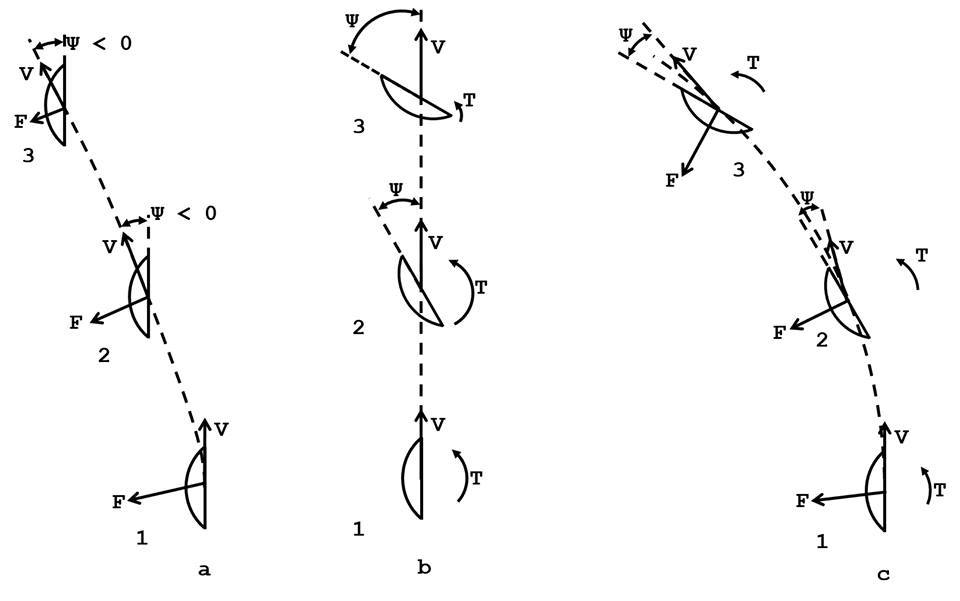
\includegraphics[scale=0.3]{imagenes/3-boomerang/TresCasos.png}
		\caption{a) Solo la fuerza F actúa. b) Solo el par T actúa. c) Actua el par T y la fuerza F. V es la velocidad de avance. $\Psi$ es el ángulo de incidencia. 1,2,3: posiciones sucesivas en vista superior.}
		\label{fig9}
		\end{center}
		\end{figure}

	Caso a: Solo la fuerza neta F actúa, el par neto T es despreciable. El boomerang adquiere una velocidad hacia la izquierda, adicional a su velocidad de avance original. Su plano de rotación permanece paralelo a si mismo. Esto resulta en un angulo de incidencia cada vez más negativo: $\Psi$<0. Conforme esto sucede, la fuerza F decrece hasta que se desvanece y el boomerang finalmente vuela en linea recta a una $\Psi$ constante menor a cero.

	Caso b: Solo el par neto T actua, la fuerza neta F es despreciable. El boomerang vuela en linea recta a velocidad constante.  Mientras tanto, la precesión rota al boomerang en contra de las manecillas del reloj respecto a un eje imaginario perpendicular al suelo. Esto incrementa el ángulo de incidencia $\Psi$ cada vez más. Si T no se desvanece antes de que $\Psi$ sea igual a 90 grados, el boomerang finalmente se moverá perpendicular a su trayectoria de vuelo.

	Caso c: Actua tanto el par T como la fuerza F. En un buen boomerang, estos efectos están balanceados. Si el par T causa un incremento de $\Psi$, la fuerza F también incrementará, empujando el boomerang hacia la izquierda, restringiendo el incremento excesivo de $\Psi$. El resultado es una trayectoria de vuelo curva.

	Si el boomerang se mueve en un plano no vertical, es decir, con un ángulo menor a 90 grados respecto a un eje imaginario del CM hacia su parte posterior, la fuerza F puede tener una componente hacia arriba que contrarreste el peso y mantenga al boomerang en el aire por más tiempo.

	Por otro lado, es posible inclinar una ala de cualquier sección transversal en un ángulo, denotado por ``ángulo de ataque'', tal que la fuerza de empuje resultante sea cero (Fig. \ref{fig10}.a) presentando solo un poco de arrastre. Para una sección transversal plana esta dirección es obviamente paralela al plano del ala. Para alas con un lado más convexo en la parte superior esta sección corresponde a una inclinación aparentemente negativa. A cualquier otro ángulo de ataque, el ala va a generar fuerza de empuje (vease Fig. \ref{fig10}.b). El ángulo ($\alpha$) entre la inclinación de empuje cero y la inclinación actual es llamada ``sección de angulo de ataque efectivo''. Si este ángulo $\alpha$ es suficientemente pequeño (digase $|\alpha| <= 10 grados$), el empuje es aproximadamente proporcional a este.

		\begin{figure}[ht]
		\begin{center}
		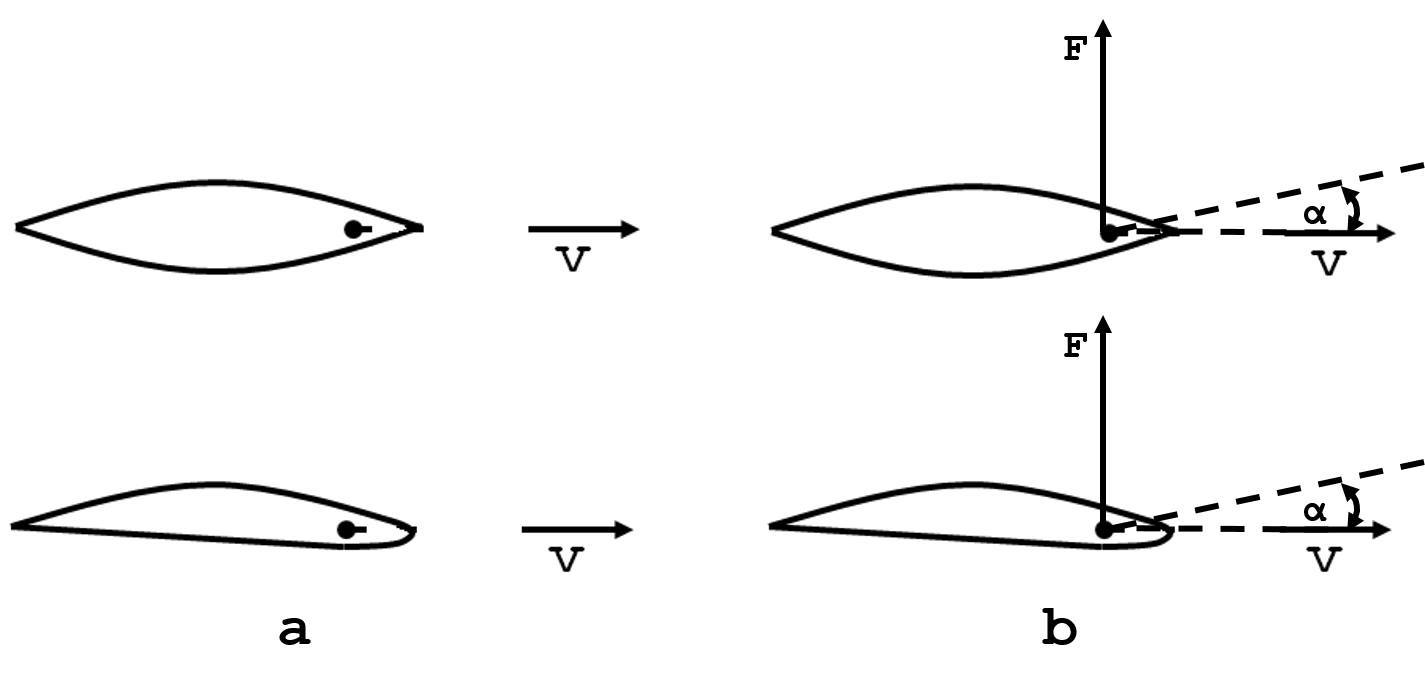
\includegraphics[scale=0.2]{imagenes/3-boomerang/atackangle.jpg}
		\caption{Ángulo de ataque.}
		\label{fig10}
		\end{center}
		\end{figure}

		\subsection{Más de la mecánica del boomerang.}

	En esta sección trataremos dos temas:
    	\begin{enumerate}[A)]
		\item El tamaño de la trayectoria del booerang.
		\item El recostamiento del boomerang.
		\end{enumerate}

	A: El tamaño de la trayectoria del boomerang.

	Supongase que un boomerang vuela aproximadamente a lo largo de un círculo horizontal, con su plano de rotación vertical, y con un ángulo de incidencia $\Psi$ pequeño y constante. Sea la velocidad de avance V ($\frac{m}{s}$) y su velocidad angular $\omega$ ($\frac{rad}{s}$). Sea una velocidad de precesión $\Omega$ ($\frac{rad}{s}$) relacionada con el par T y w de acuerdo con la formula:

		\begin{equation}
		\Omega = \frac{T}{I\omega}
		\label{ec1}
		\end{equation}  %% 17.1


	donde I es el momento de inercia del objeto respecto a su eje de rotación.

		\begin{figure}[ht]
		\begin{center}
		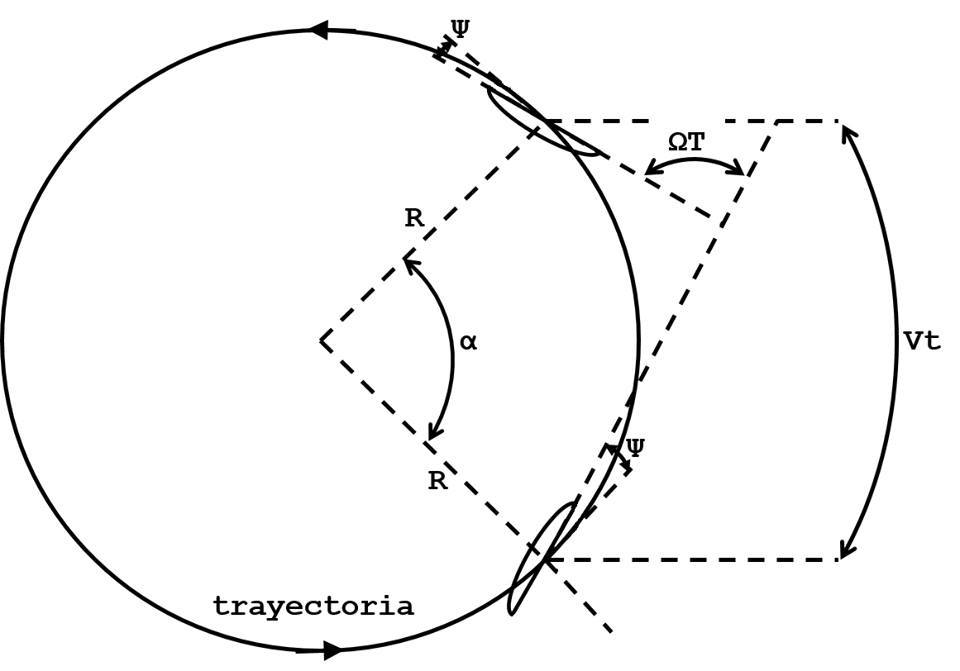
\includegraphics[scale=0.3]{imagenes/3-boomerang/TrayectoriaCircular.png}
		\caption{Posición del boomerang en dos instantes, con t segundos de separación (vista superior).}
		\label{fig11}
		\end{center}
		\end{figure}


	Sea R el radio de la trayectoria circular (vease Fig. \ref{fig11}). En un tiempo t, el boomerang describe un arco de longitud $Vt$ metros. El ángulo, visto desde el centro de la trayectoria se denota como $\alpha$, de tal manera que la longitud del arco es $\alpha R$. Por tanto: $\alpha R = Vt$. En el mismo intervalo de tiempo, el boomeran realiza un movimiento de precesión generando un ángulo de $\Omega t$. Si el ángulo de incidencia $\Psi$ (angulo entre el plano del boomerang y la trayectoria de vuelo) es constante, tenemos que $\Omega T = \alpha$. Entonces $\Omega t R = V t$ y

		\begin{equation}
		\Omega R = V
		\label{ec2}
		\end{equation} %% 17.2

	Para hacer volar un boomerang a lo largo de una trayectoria curva de radio R, una fuerza centrípeta (dirigida hacia el centro del círculo) es requerida de magnitud $\frac{m V^{2}}{R}$, donde m es la masa del boomerang. Esta fuerza, por supuesto, es suprimida por la fuerza aerodinámica F, por tanto

		\begin{equation}
		F = \frac{m V^{2}}{R}
		\label{ec3}
		\end{equation} %% 17.4

	Para el radio R de la trayectoria de vuelo obtenemos

		\begin{equation}
		R = \frac{mV^{2}}{F}
		\label{ec4}
		\end{equation} %% 17.4

	Además, de (17.1) y (17.2) tenemos que

		\begin{equation}
		R = \frac{V}{Omega} = \frac{IwV}{T}
		\label{ec5}
		\end{equation} %% 17.5

	De (17.4) y (17.5) se obtiene la condición

		\begin{equation}
		\frac{T}{Iw} = \frac{F}{mV}
		\label{ec6}
		\end{equation} %% 17.6

	Ambos T $\&$ F dependen del ángulo de incidencia $\Psi$. Por tanto, $\Psi$ tiene un valor tal que (\ref{ec6}) se satisface. Enfatizamos, sin embargo, que este forma de vuelo no siempre es posible.

	Consideremos ahora el caso en que el boomerang es arrojado a una velocidad mayor, de tal manera que V y $\omega$ incrementan. De acuerdo con (\ref{ec4}), R parece incrementar en función de V. Por otro lado, F también incrementa en función de V. Si asumimos que la razón $\frac{\omega}{V}$ es la misma en cada lanzamiento, y, además, $\Psi$ permanece igual, entonces F resulta proporcional a $V^{2}$ (o a $\omega^{2}$ o a $\omega V$) de acuerdo con la teoría aerodinámica. Por tanto, R permanece sin cambio de acuerdo a (\ref{ec4}). Alternativamente se puede utilizar (\ref{ec5}) para notar que T es proportcional a $\omega V$. En conclusión, esto significa que el radio de trayectoria de vuelo es independiente de cuan rápido es arrojado el boomerang.

	En cierto sentido cada boomerang tiene su propio radio de trayectoria de vuelo. Si un boomerang es elaborado con mayor masa, de tal manera que m y I son incrementados, pero su forma permanece igual que antes, (\ref{ec4}) y (\ref{ec5}) muestran que el radio de trayectoria de vuelo se incrementa.


		B: El recostamiento del boomerang.

	Generalmente, la parte frontal del boomerang experimenta más empuje hacia la izquierda que la parte posterior. Esto es causado principalmente por efectos estela. El aire, conforme pasa por el boomerang, gradualmente adquiere una velocidad inducida hacia la derecha porque es empujado hacia la derecha por las alas del boomerang. La parte posterior del boomerang no experimente aire “virgen”, sino aire moviendose ligeramente hacia la derecha, por lo que esta parte experimenta menos empuje. Esto causa que el par T obtenga una componente que trata de rotar el boomerang con su parte frontal a la izquierda.. La precesión entonces gira el boomerang en su parte superior a la derecha. El resultado es visible como “recostamiento”. En otras palabras, el epje del par T no es exactamente horizontal, como se indica en la Fig. \ref{fig7}, sino rotado un poco hacia arriba. La precesión, por tanto, actua respecto a un eje no exactamente vertical, sino rotado un poco hacia adelante.

	Considerese un boomerang tradicional diestro (vease Fig. \ref{fig1}.c). Ambos brazos (1 y 2), experimentan un empuje máximo hacia la izquierda cuando apuntan hacia arriba. En el caso del brazo 1, la posición de la fuerza máxima está por delante del centro de masa, y de forma contraria para el brazo 2. Si el empuje en el brazo 1 es incrementado proporcionandole una sección transversal adecuada, o más inclinación, y/o el empuje en el brazo 2 es decrementado de forma similar, resulta un componente de par tratando de rotar el boomeran por su parte frontal hacia la izquierda, lo que resulta en recostamiento por precesión.

    %\section{Aerodinámica de los Boomerangs}

	\subsection{Ecuaciones de movimiento del Boomerang}

	 En las siguientes siguientes subsecciones se mostrarán las ecuaciones de movimiento del boomerang, en las cuales las fuerzas aerodinámicas se dejan sin especificar. Las magnitudes de esas fuerzas deben ser derivadas ya sea por modelos teóricos o por mediciones.

	 Un boomerang es considerado como un cuerpo rígido cuyo comportamiento es parecido a un trompo girando rápidamente. Se asume que gira rápidamente  al rededor del eje principal a través del centro de masa en donde se encuetra el mayor momento de inercia. La simplifición de las ecuaciones dinámicas de movimiento del boomerang se debe a que las fuerzas actuando en él son promediadas ó suavizadas.

	 La justifiación del suavizado puede ser basado en la suposición de que las variaciones ó fluctuaciones durante el vuelo del boomerang son rápidas ó lentas. Las variaciones rápidas tienen características de tiempo del orden de un periodo de rotacion ó menos, mientras que las variaciones lentas son más grandes que el periodo de rotación.

	 Una desventaja de suavizar las ecuaciones de moviemiento son, por supuesto, la información perteneciente a las variaciones de las cantidades mecánicas y aerodinámicas son perdidas.


	\subsubsection{Ecuaciones de movimiento I}

	A lo largo de el cálculo de las ecuaciones de movimiento del boomerang se considera a este como un cuerpo rígido, además, se considera que el vector del momento angular es aproximadamente paralelo al eje principal del cuerpo, con la mayor cantidad de momento de inercia.

		Se definirán los siguentes sistemas coordenados utilizando la regla de la mano derecha:

		\begin{enumerate}
		\item (X,Y,Z), Sistema fijo inercial con respecto al cual se desea calcular la trayectoria de vuelo del boomerang.
		\item (1,2,3), Sistem fijo del boomerang. El origen del sistema esta en el centro de masa del boomerang.
		\item (x,y,z), Sistema parcialmente fijo al boomerang. El eje z coincide con el eje 3. La proyección de la velocidad del centro de masa del boomerang esta sobre el plano (x,y) y apunto en direccion negativa del eje x. Nuevamente el origen del sistema coordenado se ubica en el centro de masa del boomerang.
		\end{enumerate}

		\begin{figure}[ht]
		\begin{center}
		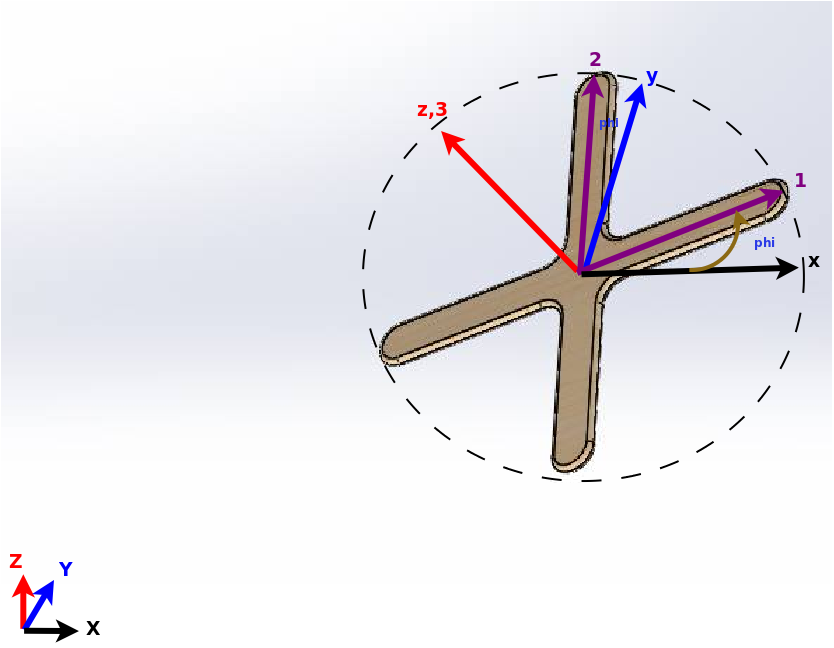
\includegraphics[scale=0.15]{imagenes/3-boomerang/sistemas_coordenados.png}
		\caption{Sistemas coordenados (X,Y,Z),(x,y,z),(1,2,3).}
		\label{fig12}
		\end{center}
		\end{figure}


	Para comenzar con el análisis, primero se derivarán las ecuaciones de movimiento del boomerang con respecto al sistema (x,y,z), desde que el sistema esta directamente relacionado con el estado de movimiento del boomerang con respecto al aire. El sistema (x,y,z) rota a una velocidad angular:


		\begin{equation}
		\vec{\Omega} = (\Omega_{x},\Omega_{y},\Omega_{z})
		\label{ec7}
		\end{equation} %% pag 80

	$\Omega_{z}$ esta determinada cinemáticamente por el hecho de que la componente ``y'' de la velocidad del centro de masa del boomerang es cero por definición. El movimiento del boomerang se puede separar en 2 partes:

		\begin{enumerate}
		\item{Movimiento del centro de masa.}
		\item{Movimiento del cuerpo con respecto a su centro de masa.}
		\end{enumerate}

	\subsubsection{Movimiento del centro de masa.}

	La velocidad del centro de masa del boomerang esta dada por:

		\begin{equation}
		\vec{V} = (V_{x},V_{y},V_{z})
		\label{ec8}
		\end{equation} %% pag 81


	donde las componentes están dadas en las direcciones x,y,z respectivamente. Por la deficición del sistema (x,y,z), tenemos:

		\begin{subequations}
		\begin{align}
    	V_{x} < 0 \\
		V_{y} = 0
		\end{align}
		\label{ec9}
		\end{subequations} %% pag 81

	Además dada la fuerza $\vec{F}$ como la fuerza resultante actuando sobre el boomerang, m la masa del boomerag, se tiene la fuerza expesada en relación del cambio del momento lineal:

		\begin{subequations}
		\begin{align}
		\vec{F} = \dot{\vec{P}} \\
		\vec{P} = m\vec{V}
		\end{align}
		\label{ec10}
		\end{subequations} %% pag 81

	Se llega a lo siguiente:

		\begin{equation}
		\vec{F} = {d\vec{p}\over dt} = \left({d\vec{p}\over dt} \right)^{\prime} + \vec{\Omega} \times \vec{p}
		\label{ec11}
		\end{equation} %% pag 81

	Utilizando (\ref{ec9}), tenemos:

		\begin{equation}
		\begin{bmatrix}
  		F_{x}\\
  		F_{y}\\
  		F_{z}
  		\end{bmatrix} =
  		m \dot{\vec{V}} + \vec{\Omega} \times m \vec{V} =
  		m \begin{bmatrix}
  		\begin{matrix}
  		\dot{V_{x}}\\
  		\dot{V_{y}}\\
  		\dot{V_{z}}\\
  		\end{matrix}
		+
		\begin{pmatrix}
        \Omega_{x}\\
        \Omega_{y}\\
        \Omega_{z}\\
		\end{pmatrix}
    	\times
		\begin{pmatrix}
        V_{x}\\
        V_{y}\\
        V_{z}\\
   		\end{pmatrix}
  		\end{bmatrix}
  		=
  		m \begin{bmatrix}
  		\begin{matrix}
  		\dot{V_{x}}\\
  		\dot{V_{y}}\\
  		\dot{V_{z}}\\
  		\end{matrix}
		+
		\begin{pmatrix}
        \Omega_{y}V_{z}-\Omega_{z}V_{y}\\
        \Omega_{x}V_{z}-\Omega_{z}V_{x}\\
        \Omega_{x}V_{y}-\Omega_{y}V_{x}\\
   		\end{pmatrix}
  		\end{bmatrix}
		\label{ec12}
		\end{equation} %% pag 81

	resultando:

		\begin{equation}
		\begin{bmatrix}
  		F_{x}\\
  		F_{y}\\
  		F_{z}
	  	\end{bmatrix} =
  		m \begin{bmatrix}
  		\begin{matrix}
  		\dot{V_{x}} + \Omega_{y}V_{z}\\
	    \Omega_{x}V_{z}-\Omega_{z}V_{x} \\
  		\dot{V_{z}}-\Omega_{y}V_{x}\\
   		\end{matrix}
  		\end{bmatrix}
		\label{ec13}
		\end{equation} %% pag 81

	La segunda ecuación de (\ref{ec13}) determina el valor de $\Omega_{z}$. Las solución exacta de las ecuaciones de (\ref{ec13}) son remplazadas por las ecuaciones  aproximadas o suavizadas:

		\begin{equation}
		\begin{bmatrix}
  		\bar{F_{x}}\\
  		\bar{F_{y}}\\
  		\bar{F_{z}}
  		\end{bmatrix} =
  		m \begin{bmatrix}
  		\begin{matrix}
  		\dot{\bar{V_{x}}} + \bar{\Omega_{y}}\bar{V_{z}}\\
    	\bar{\Omega_{x}}\bar{V_{z}}-\bar{\Omega_{z}}\bar{V_{x}} \\
  		\dot{\bar{V_{z}}}-\bar{\Omega_{y}}\bar{V_{x}}\\
   		\end{matrix}
  		\end{bmatrix}
		\label{ec14}
		\end{equation} %% pag 81

	En las ecuaciones (\ref{ec14}) las barras denotan las cantidades suavizadas. Las fuerzas $\bar{F_{x}}$, $\bar{F_{y}}$, $\bar{F_{z}}$ son fuerzas promediadas ó suavizadas. Las demás cantidades son resueltas por completo, por las ecuaciones de movimiento. La solución no será exacta desde que (\ref{ec14}) no son exactas. Pero proporcionan una aproxación razonable para el movimiento del centro de masa.

		\subsubsection{Movimiento con respecto al centro de masa.}

	Dada la velocidad angular del boomerang $\vec{\omega} = (\omega_{x},\omega_{y},\omega_{z})$ . Por definición del sistema x,y,z:

		\begin{subequations}
		\begin{align}
		\Omega_{x} = \omega_{x} \\
		\Omega_{y} = \omega_{y}
		\end{align}
		\label{ec15}
		\end{subequations} %% pag 82

	Dado $\bar{T}$ como el par resultante actuando en el boomerang y $\vec{L}$ el vector del momento angular del boomerang:

		\begin{equation}
		\vec{T} = \dot{\vec{L}}
		\label{ec16}
		\end{equation} %% pag 82

	y

	    \begin{equation}
		\vec{T} = {d\vec{L}\over dt} = \left({d\vec{L}\over dt} \right)^{\prime} + \vec{\Omega} \times \vec{L}
		\label{ec17}
		\end{equation} %% pag 82

	Resultando:

		\begin{equation}
		\begin{bmatrix}
  		T_{x}\\
  		T_{y}\\
  		T_{z}
  		\end{bmatrix} =
  		\begin{bmatrix}
  		\begin{matrix}
  		\dot{L_{x}}\\
  		\dot{L_{y}}\\
  		\dot{L_{z}}\\
  		\end{matrix}
		+
        \begin{pmatrix}
        \Omega_{x}\\
        \Omega_{y}\\
        \Omega_{z}
		\end{pmatrix}
    	\times
        \begin{pmatrix}
        L_{x}\\
        L_{y}\\
        L_{z}
		\end{pmatrix}
  		\end{bmatrix}
  		=
  		m \begin{bmatrix}
  		\begin{matrix}
  		\dot{L_{x}}\\
  		\dot{L_{y}}\\
  		\dot{L_{z}}\\
  		\end{matrix}
		+
	    \begin{pmatrix}
        \Omega_{y}L_{z}-\Omega_{z}L_{y}\\
        \Omega_{x}L_{z}-\Omega_{z}L_{x}\\
        \Omega_{x}L_{y}-\Omega_{y}L_{x}
		\end{pmatrix}
  		\end{bmatrix}
		\label{ec18}
		\end{equation} %% pag 81

	Para obtener $L_{x}, L_{y}$ y $L_{z}$ es necesario considerar el sistema (1,2,3). Tomando en cuenta que el eje 3 coincide con el eje z, se observa un ángulo $\phi$ en el plano (x,y) con el plano (1,2), entonces:

    	\begin{subequations}
    	\begin{align}
    	\dot{\phi} = \omega_{3}-\Omega_{z}\\
    	\omega_{3} = \omega_{z}
		\end{align}
		\label{ec19}
		\end{subequations} %% pag 82

	Los componentes del momento angular con respecto al sistema (1,2,3) están relacionados con el momento de inercia prinicipal de la siguiente manera:

		\begin{subequations}
    	\begin{align}
    	L_{1} = I_{1}\Omega_{1}\\
    	L_{2} = I_{2}\Omega_{2}\\
    	L_{3} = I_{3}\Omega_{3}
		\end{align}
		\label{ec20}
		\end{subequations} %% pag 82

	La matriz de transformación del sistema (1,2,3) al sistema (x,y,z) y viceversa esta dado por:

		\begin{equation}
    	R = \bordermatrix{~ & 1 & 2 & 3 \cr
        x & cos(\phi) & -sen(\phi) & 0 \cr
        y & sen(\phi) &  cos(\phi) & 0 \cr
        z & 0       &  0       & 1 \cr }
    	\label{ec21}
    	\end{equation}

    Por lo que obtenemos:

		\begin{equation}
		\begin{bmatrix}
  		{L_{x}}\\
  		{L_{y}}\\
  		{L_{z}}
  		\end{bmatrix} =
 		\begin{pmatrix}
        & cos(\phi) & -sen(\phi) & 0 \\
        & sen(\phi) &  cos(\phi) & 0 \\
        & 0       &  0       & 1
		\end{pmatrix}
    	\begin{bmatrix}
  		L_{1}\\
  		L_{2}\\
  		L_{3}
  		\end{bmatrix}
  		=
    	\begin{bmatrix}
  		cos(\phi) L_{1} - sen(\phi) L_{2} \\
  		sen(\phi) L_{1} + cos(\phi) L_{2} \\
  		L_{3}
  		\end{bmatrix}
  		=
    	\begin{bmatrix}
  		cos(\phi) I_{1} \omega_{1} - sen(\phi) I_{2} \omega_{2} \\
  		sen(\phi) I_{1} \omega_{1} + cos(\phi) I_{2} \omega_{2} \\
  		I_{3} \omega_{3}
  		\end{bmatrix}
		\label{ec22}
		\end{equation} %% pag 81

		\begin{equation}
		\begin{bmatrix}
  		{\omega_{1}}\\
  		{\omega_{2}}\\
  		{\omega_{3}}
  		\end{bmatrix} =
 		\begin{pmatrix}
        & cos(\phi) & sen(\phi) & 0 \\
        & -sen(\phi) &  cos(\phi) & 0 \\
        & 0       &  0       & 1
		\end{pmatrix}
    	\begin{bmatrix}
  		w_{x}\\
  		w_{y}\\
  		w_{z}
  		\end{bmatrix}
  		=
    	\begin{bmatrix}
  		cos(\phi) w_{x} + sen(\phi) w_{y}\\
   		-sen(\phi) w_{x} + cos(\phi) w_{y}\\
  		\omega_{z}
  		\end{bmatrix}
		\label{ec23}
		\end{equation} %% pag 81

	Sustiyendo (\ref{ec23}) en (\ref{ec22}):

    	\begin{equation}
		\begin{bmatrix}
  		{L_{x}}\\
  		{L_{y}}\\
  		{L_{z}}
  		\end{bmatrix} =
 		\begin{pmatrix}
        \frac{1}{2}(I_{1}+I_{2})\omega_{x} + \frac{1}{2}(I_{1}-I_{2})(\omega_{x}cos(2\phi)+\omega_{y}sen(2\phi)) \\
        \frac{1}{2}(I_{1}+I_{2})\omega_{y} + \frac{1}{2}(I_{1}-I_{2})(\omega_{x}sen(2\phi)+\omega_{y}cos(2\phi)) \\
        \omega_{z}
		\end{pmatrix}
		\label{ec24}
		\end{equation} %% pag 81

	Utilizando (\ref{ec19}) obtenemos por diferencición de (\ref{ec22}):

		\begin{equation}
		\begin{bmatrix}
	  	\dot{L_{x}}\\
  		\dot{L_{y}}\\
  		\dot{L_{z}}
  		\end{bmatrix} =
 		\begin{pmatrix}
 		I_{1}\dot{\omega_{1}}cos(\phi)-I_{2}\dot{\omega_{2}}sen(\phi)+(\omega_{3}-\Omega_{z})(-I_{1}\omega_{1}sin(\phi)+I_{2}\omega_{2}cos(\phi))\\
   		I_{1}\dot{\omega_{1}}sin(\phi)+I_{2}\dot{\omega_{2}}cos(\phi)+(\omega_{3}-\Omega_{z})(I_{1}\omega_{1}cos(\phi)-I_{2}\omega_{2}sin(\phi))\\
        I_{3}\dot{\omega_{3}}
		\end{pmatrix}
		\label{ec25}
		\end{equation} %% pag 81

	y por diferenciación de (\ref{ec23}) se obtiene:

		\begin{equation}
		\begin{bmatrix}
  		\dot{\omega_{1}}\\
  		\dot{\omega_{2}}\\
  		\dot{\omega_{3}}
  		\end{bmatrix} 	=
    	\begin{bmatrix}
  		\dot{\omega_{x}}cos(\phi) + \dot{\omega_{y}}sen(\phi) + (\omega_{z}-\Omega_{z})(-w_{x} sen(\phi) + w_{y}cos(\phi)) \\
  		-\dot{\omega_{x}}sen(\phi) + \dot{\omega_{y}}cos(\phi) + (\omega_{z}-\Omega_{z})(-w_{x} cos(\phi) - w_{y}sen(\phi)) \\
  		\dot{\omega_{z}}
  		\end{bmatrix}
		\label{ec26}
		\end{equation} %% pag 81

	Sustituyendo (\ref{ec23}) y (\ref{ec26}) en (\ref{ec25}):

		\begin{equation}
		\begin{bmatrix}
	  	\dot{L_{x}}\\
  		\dot{L_{y}}\\
  		\dot{L_{z}}
  		\end{bmatrix} =
 		\begin{pmatrix}
 		\frac{1}{2}(I_{1}+I_{2})\dot{\omega{x}} + \frac{1}{2}(I_{1}-I_{2})(-\dot{\omega_{x}}cos(2\phi)+\dot{\omega_{y}}sen(2\phi))+ (I_{1}-I_{2})(\omega_{z}-\Omega_{z})(-{\omega_{x}}sen(2\phi)+{\omega_{y}}cos(2\phi))\\
 		\frac{1}{2}(I_{1}+I_{2})\dot{\omega{y}} + \frac{1}{2}(I_{1}-I_{2})( \dot{\omega_{x}}sen(2\phi)+\dot{\omega_{y}}cos(2\phi))+ (I_{1}-I_{2})(\omega_{z}-\Omega_{z})({\omega_{x}}cos(2\phi)+{\omega_{y}}sen(2\phi))\\
 		I_{3}\dot{\omega_{3}}
		\end{pmatrix}
		\label{ec27}
		\end{equation} %% pag 81

	Utlizando (\ref{ec22})	y (\ref{ec27}) en (\ref{ec18}) y recurriendo a (\ref{ec15}):

		\begin{equation}
		\begin{bmatrix}
	  	{T_{x}}\\
  		{T_{y}}\\
  		{T_{z}}
  		\end{bmatrix} =
  		\begin{pmatrix}
 		\begin{smallmatrix}
        \frac{1}{2}(I_{1}+I_{2})\dot{\omega_{x}} - \frac{1}{2}(I_{1}+I_{2})\omega_{y}\Omega_{z} + I_{3}\omega_{z}\omega_{y} + \frac{1}{2}(I_{1}-I_{2})(-\dot{\omega_{x}}cos(2\phi)+\dot{\omega_{y}}sen(2\phi)) + \frac{1}{2}(I_{1}-I_{2})(2\omega_{z}-\Omega_{z})(-\omega_{x}sen{2\phi}+\omega_{y}cos{2\phi})\\
        \frac{1}{2}(I_{1}+I_{2})\dot{\omega_{y}} + \frac{1}{2}(I_{1}+I_{2})\omega_{x}\Omega_{z} - I_{3}\omega_{z}\omega_{y} + \frac{1}{2}(I_{1}-I_{2})(-\dot{\omega_{x}}sen(2\phi)+\dot{\omega_{y}}cos(2\phi)) + \frac{1}{2}(I_{1}-I_{2})(2\omega_{z}-\Omega_{z})(\omega_{x}cos{2\phi}+\omega_{y}sen{2\phi})\\
        I_{3}\dot{\omega_{z}}+(I_{1}-I_{2})[(\omega_{x}^{2}+\omega_{y}^{2})sen(2\phi)-\omega_{x}\omega_{y}cos(2\phi)]
		\end{smallmatrix}
  		\end{pmatrix}
		\label{ec28}
		\end{equation} %% pag 81

	Para nuestro boomerang se cumple $I_{1}=I_{2}=I_{12}$, la ecuación (\ref{ec28}) se reduce a:

		\begin{equation}
		\begin{bmatrix}
	  	{T_{x}}\\
  		{T_{y}}\\
  		{T_{z}}
  		\end{bmatrix} =
  		\begin{pmatrix}
        I_{12}\dot{\omega_{x}} + (I_{3}\omega_{z}-I_{12}\Omega_{z})\omega_{y}\\
        I_{12}\dot{\omega_{y}} - (I_{3}\omega_{z}-I_{12}\Omega_{z})\omega_{x}\\
        I_{3}\dot{\omega_{z}}
  		\end{pmatrix}
		\label{ec29}
		\end{equation} %% pag 81

	las cuales son las ecuaciones para una vista simétrica cn respecto al sistema (x,y,z). Hasta este punto todas las ecuaciones son exactas. Las ecuaciones (\ref{ec28}) se suavizan de la siguiente manera:

		\begin{equation}
		\begin{bmatrix}
	  	\bar{T_{x}}\\
  		\bar{T_{y}}\\
  		\bar{T_{z}}
  		\end{bmatrix} =
  		\begin{pmatrix}
        I_{12}\bar{\dot{\omega_{x}}} + (I_{3}\bar{\omega_{z}}-I_{12}\bar{\Omega_{z}})\bar{\omega_{y}}\\
        I_{12}\bar{\dot{\omega_{y}}} - (I_{3}\bar{\omega_{z}}-I_{12}\bar{\Omega_{z}})\bar{\omega_{x}}\\
        I_{3}\bar{\dot{\omega_{z}}}
  		\end{pmatrix}
		\label{ec30}
		\end{equation} %% pag 81

	Una segunda simplificación puede ser echa, para los boomerang que giran rápidamente, generalmente se tiene:

		\begin{subequations}
    	\begin{align}
    	\| \bar{\omega_{x}} \| , \| \bar{\omega_{x}} \|, \| \bar{\Omega_{x}} \| << \| \bar{\omega_{z}} \| \\
    	\| \bar{\dot{\omega_{x}}} \| << \| \bar{\omega_{y}}\bar{\omega_{z}} \| , \| \bar{\dot{\omega_{y}}} \| << \| \bar{\omega_{x}}\bar{\omega_{z}} \|
    	\end{align}
		\label{ec31}
		\end{subequations} %% pag 82

	De esta manera se obtiene una aproximación de (\ref{ec30}):

		\begin{equation}
		\begin{bmatrix}
	  	\bar{T_{x}}\\
  		\bar{T_{y}}\\
  		\bar{T_{z}}
  		\end{bmatrix} =
  		\begin{pmatrix}
         I_{3}\bar{\omega_{z}}\bar{\omega_{y}}\\
        -I_{3}\bar{\omega_{z}}\bar{\omega_{x}}\\
        I_{3}\bar{\dot{\omega_{z}}}
  		\end{pmatrix}
		\label{ec32}
		\end{equation}

	Las ecuaciones (\ref{ec14}) y (\ref{ec32}) serán utilizadas para el cálculo de la trayectoria del vuelo del boomerang.

	\subsubsection{Ecuaciones de movimiento II}

	Las ecuaciones de movimiento de un boomerang respecto al sistema coordenado (x, y, z) son dadas por las ecuaciones (\ref{ec14}) y (\ref{ec32}) , pero ahora usaremos las variables suavizadas o promediadas exclusivamente omitiendo las barras superiores.

	En esta sección obtendremos las ecuaciones de movimiento respecto al sistema inercial fijo (X, Y, Z), en el cual el eje Z apunta verticalmente hacia arriba y el plano  (Y, Z) es horizontal. La relación entre este sistema de referencia y el sistema (x, y, z) es dada por los angulos de euler $\phi$, $\eta$ y $\vartheta$ como se muestra en la Fig. (\ref{fig13}), donde, por definición $0\le \vartheta \le \pi$.

		\begin{figure}[ht]
		\begin{center}
		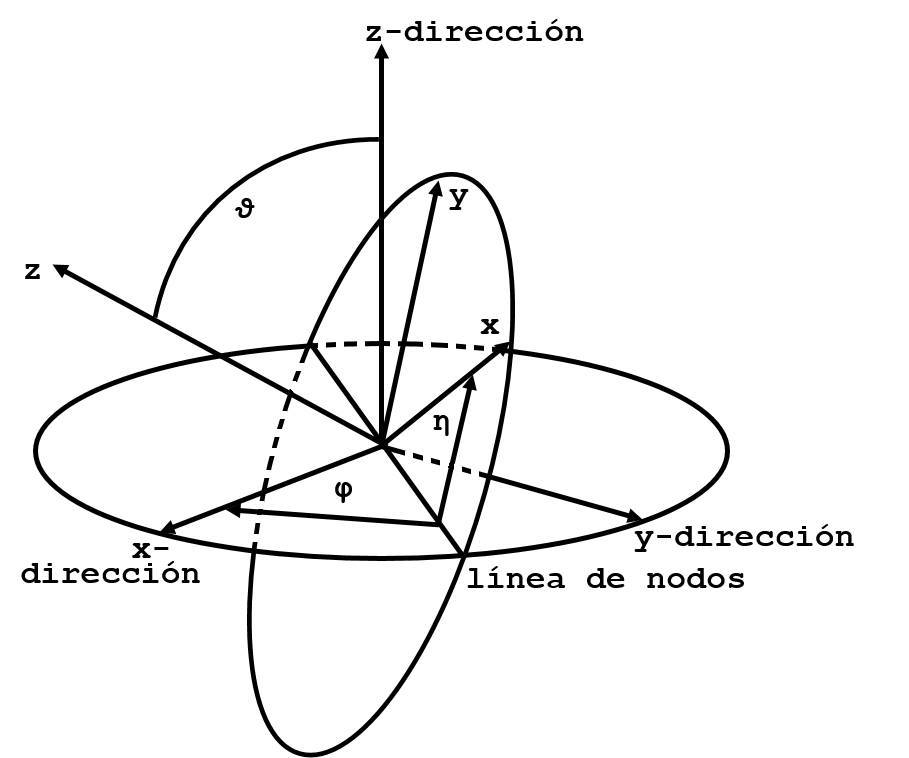
\includegraphics[scale=0.3]{imagenes/3-boomerang/euler_angles.png}
		\caption{Angulos de euler definiendo la relacion entre los sistemas coordenados (x, y, z) y (X, Y, Z).}
		\label{fig13}
		\end{center}
		\end{figure}

	La transformación que lleva un vector en (x, y, z) a su representación en el sistema de referencia (X, Y, Z) es la siguiente:

		\begin{equation}
  		\bordermatrix{ ~ & x & y & z \cr
		X & cos { \eta } cos { \varphi -cos { \vartheta } sen { \varphi } sen { \eta } } & -sen { \eta } cos { \varphi } -cos { \vartheta } sen { \varphi } cos { \eta } & sen { \vartheta } sen { \varphi } \cr
		Y & cos { \eta } sen { \varphi } +cos { \vartheta } cos { \varphi } sen { \eta } & -sen { \eta } sen { \varphi } +cos { \vartheta } cos { \varphi } cos { \eta } & -sen { \vartheta } cos { \varphi } \cr
		Z & sen { \vartheta } sen { \eta } & sen { \vartheta } cos { \eta } & cos { \vartheta }  \cr
		}
		\label{ec33}
		\end{equation}

	Para la velocidad angular $\vec { \Omega  }$  del sistema de referencia (x, y, z) ahora tenemos:

		\begin{equation}
		\begin{bmatrix}
		\Omega_{x} \\
		\Omega_{y} \\
		\Omega_{z}
		\end{bmatrix} =
		\begin{pmatrix}
	    \dot{\vartheta}cos{\eta + \dot{\varphi}sen{\vartheta}sen{\eta}} \\
		-\dot{\vartheta}sen{\eta}+\dot{\varphi}sen{\vartheta}cos{\eta}\\
		\dot{\eta}+\dot{\varphi}cos{\vartheta}
  		\end{pmatrix}
		\label{ec34}
		\end{equation}

		lo que lleva a:

		\begin{equation}
		\begin{bmatrix}
		\dot{\vartheta}\\
		\dot{\varphi}\\
     	\dot{\eta}
		\end{bmatrix} =
		\begin{pmatrix}
		{\Omega}_{x}cos{\eta}-{\Omega}_{y}\sin{\eta}\\
		\frac{1}{\sin{\vartheta}}({\Omega}_{x}\sin{\eta}+{\Omega}_{y}cos{\eta})\\
		{\Omega}_{z}-\frac{cos{\vartheta}}{\sin{\vartheta}}({\Omega}_{x}\sin{\eta}+{\Omega}_{y}cos{\eta})
		\end{pmatrix}
		\label{ec34}
		\end{equation}

	De (\ref{ec15}) y (\ref{ec32})  obtenemos:

		\begin{equation}
		\begin{matrix}
		\Omega_{x}={\omega}_{x}=-\frac{{T}{y}}{{I}_{3}{\omega}_{z}}\\
		\Omega_{y}={\omega}_{y}=\frac{{T}_{x}}{{I}_{3}{\omega}_{z}}\\
		\dot{\omega}_{z}=\frac{{T}_{z}}{{I}_{3}}
		\end{matrix}
		\label{ec35}
		\end{equation}

	y de (\ref{ec14}) :

		\begin{equation}
		\begin{matrix}
		\Omega_{z}=\frac{{F}_{y}}{m{V}_{x}}+\frac{{V}_{z}{\omega}_{x}}{{V}_{x}}\\
		\dot{V}_{x}=\frac{{F}_{x}}{m}-{V}_{x}{\omega}_{y}\\
		\dot{V}_{z}=\frac{{F}_{z}}{m}+{V}_{x}{\omega}_{y}
		\end{matrix}
		\label{ec36}
		\end{equation}


	Introducimos las variables V y $\Psi$  definidos por:

		\begin{equation}
		\begin{matrix}
		V_{x}=-Vcos{\Psi}\\
		V_{z}=-V\sin{\Psi}\\
		V>0,\quad\left|\Psi\right|<\cfrac{1}{2}\pi
		\end{matrix}
		\label{ec37}
		\end{equation}

	Recuerdese que $Vx<0$ y Vy = 0  son los componentes sobre los ejes x $\&$ y respectivamente de la velocidad lineal del boomerang (V), Psi es el ángulo entre la parte negativa del eje x y la dirección de la velocidad del boomerang. Llamamos a $\Psi$ el ángulo de incidencia. Entonces (\ref{ec36}) puede ser escrito como:

		\begin{equation}
		\begin{matrix}
		\Omega_{z}=-\frac{{F}_{y}}{mVcos{\Psi}}+{\omega}_{x}\tan{\Psi}\\
		\dot{V}=\frac{1}{m}(-{F}_{x}cos{\Psi}-{F}_{z}\sin{\Psi})\\
		\dot{\Psi}=\frac{1}{mV}({F}_{x}\sin{\Psi-{F}_{z}cos{\Psi}})+{\omega}_{y}
		\end{matrix}
		\label{ec38}
		\end{equation}

	Las ecuaciones (\ref{ec34}), (\ref{ec35}) y (\ref{ec38}) determinan el movimiento del boomerang y pueden combinarse formando:

		\begin{equation}
		\begin{matrix}
		\dot{\omega}_{z}=\frac{T_{y}}{{I}_{3}}\\
		\dot{V}=\frac{1}{m}(-{F}_{x}cos{\Psi}-{F}_{z}\sin{\Psi})\\
		\dot{\Psi}=\frac{1}{m }({F}_{x}\sin{\Psi-{F}_{z}cos{\Psi}})+\frac{{T}_{x}}{{I}_{3}{\omega}_{z}}
		\end{matrix}
		\label{ec39}
		\end{equation}

		\begin{equation}
		\begin{matrix}
		 {\dot{\vartheta}}_{z}=\frac{1}{{I}_{3}{\omega}_{z}}(-{T}_{y}cos{\eta}-{T}_{x}\sin{\eta})\\
		 \dot{\varphi}=\frac{1}{{I}_{3}{\omega}_{z}}\frac{1}{\sin{\vartheta}}(-{T}_{y}\sin {\eta}+{T}_{x}cos{\eta})\\
		 \dot{\eta}=-\frac{{F}_{y}}{mVcos{\Psi}}-\tan{\Psi}\frac{T_{y}}{{I}_{3}{\omega}_{z}}-\dot{\varphi} cos{\vartheta}
		\end{matrix}
		\label{ec40}
		\end{equation}

	Para la posición del centro de masa del boomerang en el sistema de referencia (X, Y, Z) tenemos simplemente:

		\begin{equation}
		\begin{matrix}
		\dot{X} = V[{-cos{\Psi}(cos{\eta}cos{\varphi}-\sin{\eta}\sin{\varphi}cos{\vartheta})-\sin{\Psi}\sin{\varphi}\sin{\vartheta}]}\quad\\
	    \dot{Y}=V[{-cos{\Psi}\left(cos{\eta}\sin{\varphi}+\sin{\eta}cos{\varphi}cos{\vartheta}\right)+\sin{\Psi}cos{\varphi}\sin{\vartheta}]}\\
	    \dot{Z}=V[{-cos{\Psi\sin{\eta}\sin{\vartheta}-\sin{\Psi}cos{\vartheta}}]}
		\end{matrix}
		\label{ec41}
		\end{equation}

	Las ecuaciones (\ref{ec39}), (\ref{ec40}) y (\ref{ec41}) deben ser integradas numericamente. Las fuerzas y pares $F_{x}$, $F_{y}$, $F_{z}$, $T_{x}$, $T_{y}$, $T_{z}$ deben ser dados como funciones conocidas del estado de movimiento del sistema. Si las condiciones iniciales son proveidas, estas nueve ecuaciones diferenciales de primer orden pueden ser resueltas para las nueve incognitas $\omega_{z}$, V, $\Psi$, $\vartheta$, $\varphi$, $\eta$, X, Y, Z como funciones del tiempo, t.

	Las ecuaciones (\ref{ec39}) y (\ref{ec40})  contienen singularidades si las variables del denominador se vuelven triviales, lo cual ocurre en los cuatro casos siguientes:

		\begin{equation}
		\begin{matrix}
	    \sin{\vartheta\rightarrow}0\\
		cos{\Psi\rightarrow}0\\
		{V\rightarrow}0\\
		{{\omega}_{z}\rightarrow}0
		\end{matrix}
		\label{ec42}
		\end{equation}

	% Consideremos los casos de uno por uno.

	\subsection{Fuerzas actuantes sobre el boomerang}

	Consideremos las siguientes suposiciones concernientes al boomerang, el medio en el cual se mueve y la gravedad:

	\begin{enumerate}
	\item El boomerang es un cuerpo rígido. Su tamaño se caracteriza por su radio a, el cual es el radio que describe el boomerang al girar sobre su centro de masa. La masa del boomerang es m, y sus momentos principales de inercia, de menor a mayor magnitud, son I$_{1}$, I$_{2}$, I$_{3}$; y su densidad promedio es $\rho$.
	\item El medio es homogeneo, isotrópico, constante en el tiempo, de extensión finita. Su densidad es $\mu$, su viscosidad cinemática es $\nu$. No se consideran efectos aerodinámicos o aerodinámicos debidos a la presencia de objetos como la tierra o arboles.
	\item La aceleración de la gravedad, $\vec{g}$, se considera constante y dirigida hacia abajo, en la dirección negativa de Z
	\end{enumerate}

	Las fuerzas actuantes sobre el boomerang son de dos tipos: fuerzas debidas a la gravedad y fuerzas debidas a la interacción con el aire, denotadas por un subíndice g y a respectivamente. Entonces:

		\begin{subequations}
    	\begin{align}
	    \vec{F}={\vec{F}}_{g}+{\vec{F}}_{a}\\
    	\vec{T}={\vec{T}}_{a}
		\end{align}
		\label{ec43}
		\end{subequations}

	Los componentes de $({\vec{F}}_{g})$ en el sistema (X, Y, Z) son:

		\begin{equation}
    	{\vec{F}}_{g}=-mg(\sin{\vartheta}\sin{\eta},\sin{\vartheta}cos{\eta},cos{\vartheta})
		\label{ec44}
		\end{equation}

	Las fuerzas hidrostáticas pueden ser tomadas en cuenta reemplazando g por:

		\begin{equation}
		{g}^{\prime}=g(1-\cfrac{{\mu}}{\rho})
		\label{ec45}
		\end{equation}

	No es tan simple obtener expresiones para las fuerzas aerodinámicas, las cuales pueden depender de:

		\begin{enumerate}[a)]
		\item Las propiedades del aire: e. g. Densidad, viscosidad, turbulencia.
		\item La forma del boomerang.
		\item el estao de movimiento del boomerang: e.g.  $\Psi$ , $\vec{\omega}$ , V.
		\item historial previo
		\end{enumerate}

	De acuerdo con los metodos de analisis dimensional, los componentes en (x, y, z) de ${\vec{F}}_{a}$ pueden ser escritos en la forma:

		\begin{equation}
		\vec{F}_{a}={\mu}_{a}{a}^{2}{V}^{2}\vec{f}(\Psi,\cfrac{V}{{\omega}_{z}a},\cfrac{{\omega}_{x}}{{\omega}_{z}},\cfrac{{\omega}_{y}}{{\omega}_{z}},\phi,Re,Historial,Forma)
		\label{ec46}
		\end{equation}

	donde todos los argumentos de  $\vec{f}$ son adimensionales. $Re=\frac{aV}{\nu}$ es un número de Reynolds. El historial representa la influencia de condiciones previas en el vuelo del boomerang. La forma denota un conjunto de parametros adimensionales que definen la forma del boomerang (no el tamaño). El factor ${V}^{2}$ en (\ref{ec46}) puede ser reemplazado por $({\omega}_{z}a)^{2}$, si se desea. ${\vec{T}}_{a}$ puede ser escrito de forma similar con un factor adicional a. Es el historial el que acarrea las mayores dificultades, ya que puede depender del completo movimiento del boomerang desde su inicio, t $=$ 0, hasta su instante presente, t $=$ tp.

	Bajo la base de muchas suposiciones, la función desconocida $\vec{f}$ en (\ref{ec46}) puede ser simplificada. Ya que trabajaremos con fuerzas promediadas (suavizadas), una enorme cantidad de simplificaciones pueden ser tomadas sobre un periodo de $\phi$ , y reemplazar el historial por uno ficticio en el cual las cantidades

		\begin{equation}
		\Psi,\cfrac{V}{{\omega}_{z}a},\cfrac{{\omega}_{x}}{{\omega}_{z}},\cfrac{{\omega}_{y}}{{\omega}_{z}},Re
		\label{ec47}
		\end{equation}

	son constantes para todo $t\le{t}_{p}$ . Esto es una aproximación cuasi-estacionaria. La situación en
  	$t={t}_{p}$, para el propósito de calcular fuerzas aerodinámicas, se supone constante para $-\infty <t\le{t}_{p}$. La parte previa de la trayectoria de vuelo del boomerang es reemplazada por una línea recta. Este historial extremadamente simplificado depende solo de la situación presente $(t={t}_{p})$, y deja de ser un conjunto de variables independientes en (\ref{ec46}), por lo que obtenemos:

		\begin{equation}
		{\vec{F}}_{a}={\mu}{a}^{2}{V}^{2}\vec{f}(\Psi,U,\cfrac{{\omega}_{x}}{{\omega}_{z}},\cfrac{{\omega}_{y}}{{\omega}_{z}},Re,Forma)
		\label{ec48}
		\end{equation}

	donde U es la raza de avance, definida como:

		\begin{equation}
		U=\frac{V}{{\omega}_{z}a}
		\label{ec49}
		\end{equation}

	La dependencia de Re no es del todo despreciable, \cite{Hess1975} mostró en experimentos en túnel de viento que tiene cierta influencia. Sin embargo las fuerzas computadas por su modelo del ala son independientes de Re. Para el propósito del cálculo de la trayectoria de vuelo del boomerang asumiremos que la influencia de este número es despreciable y por lo tanto, tenemos:

		\begin{equation}
		{\vec{F}}_{a}={\mu}{a}^{2}{V}^{2}\vec{f}(\Psi,U,\cfrac{{\omega}_{x}}{{\omega}_{z}},\cfrac{{\omega}_{y}}{{\omega}_{z}},Forma)
		\label{ec50}
		\end{equation}

	Si $\frac{{\omega}_{x}}{{\omega}_{z}}$ y $\frac{{\omega}_{y}}{{\omega}_{z}}$ son muy pequeñas, no tendrán una influencia significativa en ${\vec{F}}_{a}$ y ${\vec{T}}_{a}$ , y estos parámetros pueden ser omitidos de (\ref{ec50}(. Esta suposición no es necesaria, sin embargo, como se muestra a continuación:

		\begin{subequations}
    	\begin{align}
    	{\vec{F}}_{a}={\mu}{a}^{2}{V}^{2}{\vec{F}}_{0}(\Psi,I/U)\\
    	{\vec{T}}_{a}={\mu}{a}^{3}{V}^{2}{\vec{T}}_{0}(\Psi,I/U)
		\end{align}
		\label{ec51}
		\end{subequations}

	o, alternativamente, como:

		\begin{subequations}
    	\begin{align}
		{\vec{F}}_{a}={\mu}{a}^{4}{\omega}_{z}^{2}{\vec{F}}_{1}(\Psi,U)\\
		{\vec{T}}_{a}={\mu}{a}^{5}{\omega}_{z}^{2}{\vec{T}}_{1}(\Psi,U)
		\end{align}
		\label{ec52}
		\end{subequations}

	donde ${\vec{F}}_{0}$ y ${\vec{T}}_{0}$ o ${\vec{F}}_{1}$ y ${\vec{T}}_{1}$ también dependen de la forma del boomerang. Durante vuelos reales del boomerang, la velocidad V varía fuertemente, mientras que las variaciones relativas en la velocidad de rotación ${\omega}_{z}$ son menores al 20$\%$. Por lo tanto, parece conveniente utilizar (\ref{ec52}) en lugar de (\ref{ec51}), esto es, durante el vuelo del boomerang, las variables adimensionales ${\vec{F}}_{1}$ y ${\vec{T}}_{1}$ se comportan practicamente como ${\vec{F}}_{a}$ y ${\vec{T}}_{a}$.

	Finalmente, reconsideremos la suposición del desvanecimiento de ${ \omega }_{ x } y { \omega }_{ y }$. La restricción impuesta por esto puede ser removida. En lugar de (5.10) ahora tenemos:


	\subsection{La influencia del viento}

	La influencia del viento en el movimiento del boomerang debe de ser tomada en cuenta, esto puede incluirse fácilmente en las ecuaciones  (\ref{ec39}) y (\ref{ec40}). Se supone que el viento predominante puede ser descrito por el campo vectorial $\vec{W}(X,Y,Z,t)$  con los componentes $W_{X}$,$W_{Y}$ y $W_{Z}$ dados. Los componentes de esta velocidad con respecto al sistema (x,y,z) se obtiene por la matriz de transformación (\ref{ec33}). Por lo que la velocidad del boomerang con respecto al aire resulta:

		\begin{equation}
		\vec{V} - \vec{W} = ({Vx}-{Wx}, {-Wy}, {Vz}-{Wz}) = (-{V}cos{\Psi}-{Wx}, {-Wy}, -{V}sen{\Psi}-{Wz})
		\label{ec53}
		\end{equation}

	Desde que se trabaja con las ecuaciones suavizadas es necesario asumir que $\vec{V}-\vec{W}$ varía relativamente poco durante un periodo de giro del boomerang. Por lo tanto las flutuaciones repentinas en la velocidad del viento se descartan.

		\begin{figure}[ht]
		\begin{center}
		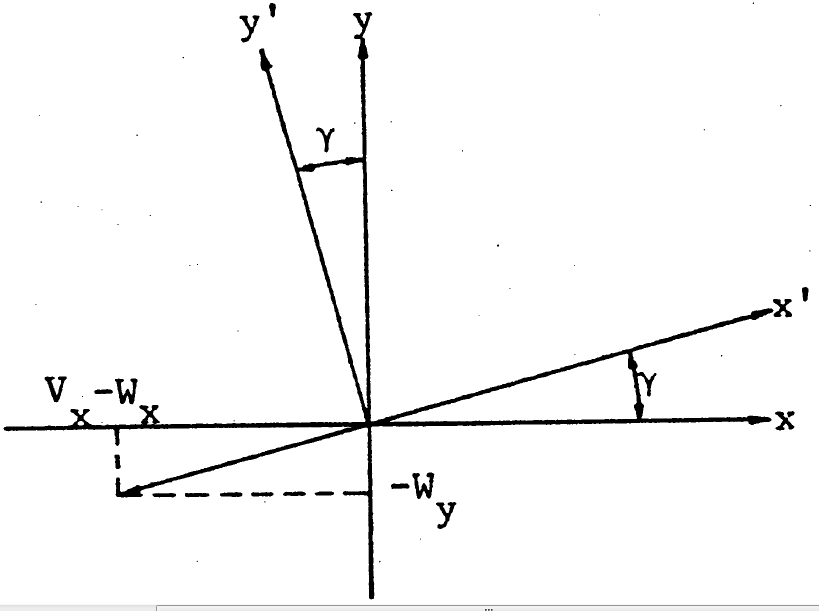
\includegraphics[scale=0.4]{imagenes/3-boomerang/vel_vient.png}
		\caption{Sistema coordenado (x,y,z) y (x$^\prime$,y$^\prime$,z$^\prime$).}
		\label{fig13}
		\end{center}
		\end{figure}

	Se introduce un nuevo sistema coordenado $(x^{\prime},y^{\prime},z^{\prime})$, de tal manera que la velocidad relativa en la dirección de $y^{\prime}$ del boomerang con respecto al bommerang desaparece. El ángulo $\gamma$ entre el eje $x$ y el eje $x^{\prime}$ esta dado por:

		\begin{equation}
		\gamma = arctan(\frac{W_{y}}{Vcos{\Psi}+W_{x}})
		\label{ec54}
		\end{equation}

	La trasformación del sistema coordenado $(x,y,z)$ al sistema coordenado $(x^{\prime},y^{\prime},z^{\prime})$ y viceversa esta determinada por:

		\begin{equation}
    	R = \bordermatrix{~ & x & y & z \cr
        x^{\prime} & cos(\gamma) & sen(\gamma) & 0 \cr
        y^{\prime} & -sen(\gamma) &  cos(\gamma) & 0 \cr
        z^{\prime} & 0       &  0       & 1 \cr }
    	\label{ec55}
    	\end{equation}

    Las componentes de la velocidad relativa del boomerang respecto al aire pueden ser reescritas por:

    	\begin{equation}
		\vec{V} - \vec{W} = (-\sqrt{(Vcos{\Psi}+W_{x})^{2}+W_{x})^{2}},0,-Vsen{\Psi}-W_{x})
		\label{ec56}
		\end{equation}

	donde las componentes estan dadas en el sistema coordenado $(x_{\prime},y_{\prime},z_{\prime})$. Agragando estos efectos a las ecuaciones de movimiento (\ref{ec39}) y (\ref{ec40}), $V$, $U$ y $\Psi$ deben ser reeplanzados por los valores relativos al movimiento del aire:

		\begin{subequations}
    	\begin{align}
		{V^{\prime}} = \sqrt{(Vcos{\Psi}+W_{x})^{2} + W_{y})^{2} + (Vsen{\Psi}+W_{z})^{2}}\\
	    = \sqrt{(V^{2} + W^{2} + 2V(W_{z}sen{\Psi} + W_{x}cos{\Psi})}
		\end{align}
		\label{ec57}
		\end{subequations}

    	\begin{equation}
		U^{\prime} = \frac{\vec{V^{\prime}}}{\omega_{z}a}
		\label{ec58}
		\end{equation}

		\begin{equation}
		{\Psi} = \arctan(\frac{W_{y}+Vsen{\Psi}}{\sqrt{(Vcos{\Psi}+W_{x})^{2} + W_{y})^{2}}})
		\label{ec59}
		\end{equation}
